\documentclass{article}
\usepackage[utf8]{inputenc}
\usepackage{amsmath}
\usepackage{amsfonts}
\usepackage{tikz}

\begin{document}

% Opcion 1: Quita la numeracion solo en esta pagina
\thispagestyle{empty} 

% Opcion 2: Descomenta la siguiente linea si quieres quitar la numeracion en TODO el documento
% \pagestyle{empty}

\begin{figure}[htbp]
\centering
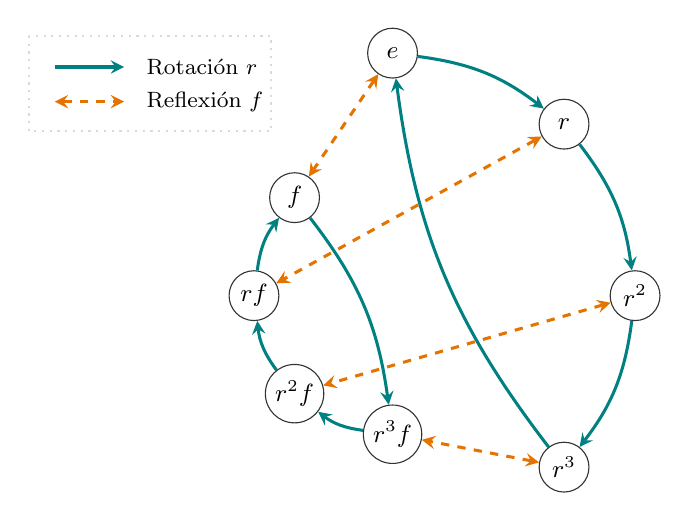
\begin{tikzpicture}[
    scale=2.2,
    % Estilo profesional para los nodos (elementos del grupo)
    nodo/.style={circle, draw=black!80, fill=white, inner sep=1.5pt, minimum size=1.8em, font=\small},
    % Estilos fijos para las aristas (generadores) con flechas elegantes
    flechaRotacion/.style={->, >=stealth, thick, color=teal, line width=1.1pt},
    flechaReflexion/.style={<->, >=stealth, thick, color=orange!90!black, dashed, line width=1.1pt}
]

    % --- DEFINICIÓN DE LOS 8 VÉRTICES (Distribución angular en un octágono) ---
    % Rotaciones (Círculo exterior)
    \node[nodo] (e)   at (90:1.4)   {$e$};
    \node[nodo] (r)   at (45:1.4)   {$r$};
    \node[nodo] (r2)  at (0:1.4)    {$r^2$};
    \node[nodo] (r3)  at (315:1.4)  {$r^3$};
    
    % Reflexiones combinadas (Círculo interior para evitar cruces)
    \node[nodo] (f)   at (135:0.8)  {$f$};
    \node[nodo] (rf)  at (180:0.8)  {$rf$};
    \node[nodo] (r2f) at (225:0.8)  {$r^2f$};
    \node[nodo] (r3f) at (270:0.8)  {$r^3f$};


    % --- ARISTAS DEL GENERADOR 'r' (Acción por la derecha g -> g*r) ---
    % Ciclo exterior: e -> r -> r^2 -> r^3 -> e
    \draw[flechaRotacion] (e) to[bend left=15] (r);
    \draw[flechaRotacion] (r) to[bend left=15] (r2);
    \draw[flechaRotacion] (r2) to[bend left=15] (r3);
    \draw[flechaRotacion] (r3) to[bend left=15] (e);

    % Ciclo interior: f -> r^3f -> r^2f -> rf -> f
    % (inversión causada por fr = r^{-1}f)
    \draw[flechaRotacion] (f) to[bend left=15] (r3f);
    \draw[flechaRotacion] (r3f) to[bend left=15] (r2f);
    \draw[flechaRotacion] (r2f) to[bend left=15] (rf);
    \draw[flechaRotacion] (rf) to[bend left=15] (f);


    % --- ARISTAS DEL GENERADOR 'f' (Reflexión: Involución bidireccional) ---
    % f^2 = e, por lo que cada conexión es una involución
    \draw[flechaReflexion] (e) -- (f);
    \draw[flechaReflexion] (r) -- (rf);
    \draw[flechaReflexion] (r2) -- (r2f);
    \draw[flechaReflexion] (r3) -- (r3f);


    % --- LEYENDA INTEGRADA DE NIVEL EDITORIAL ---
    \begin{scope}[shift={(-2.1,1.5)}]
        \draw[fill=white, draw=gray!30, dotted, thick] (0,0) rectangle (1.4,-0.55);
        \draw[flechaRotacion, ->] (0.15,-0.18) -- (0.55,-0.18) node[right, black, font=\footnotesize] {\, Rotación $r$};
        \draw[flechaReflexion, <->] (0.15,-0.38) -- (0.55,-0.38) node[right, black, font=\footnotesize] {\, Reflexión $f$};
    \end{scope}

\end{tikzpicture}

\end{figure}

\end{document}

